
% ADDING NEW DEFINITIONS -------------------------------------------- start
\definecolor{listingbg}{gray}{0.95}
\definecolor{darkgreen}{rgb}{0.0, 0.7, 0.0}
\definecolor{darkblue} {rgb}{0.0, 0.0, 0.7}
\definecolor{cyan} {rgb}{0.0, 0.4, 0.4}
\definecolor{darkred}  {rgb}{0.7, 0.0, 0.0}
\definecolor{darkorange}{rgb}{1.0, 0.49, 0.0}
\definecolor{violett}{rgb}{255, 0, 255}
\definecolor{turq}{rgb}{0.0, 0.7, 0.8}
\definecolor{fits}{rgb}{0.4, 0.1, 1}


\makeatletter
\lstdefinestyle{RAWstyle}{%
  basicstyle=\ttfamily\color{black}%
  \lst@ifdisplaystyle\scriptsize\fi}

\lstdefinestyle{PARstyle}{%
  basicstyle=\ttfamily\color{black}%
  \lst@ifdisplaystyle\scriptsize\fi}

\lstdefinestyle{DRLstyle}{%
  basicstyle=\ttfamily\color{black}%
  \lst@ifdisplaystyle\scriptsize\fi}

\lstdefinestyle{RECstyle}{%
  basicstyle=\ttfamily\color{black}%
  \lst@ifdisplaystyle\scriptsize\fi}

\lstdefinestyle{QCstyle}{%
  basicstyle=\ttfamily\color{black}%
  \lst@ifdisplaystyle\scriptsize\fi}

\lstdefinestyle{TPLstyle}{%
  basicstyle=\ttfamily\color{black}%
  \lst@ifdisplaystyle\scriptsize\fi}

\lstdefinestyle{PRODstyle}{%
  basicstyle=\ttfamily\color{black}%
  \lst@ifdisplaystyle\scriptsize\fi}

\lstdefinestyle{EXTCALIBstyle}{%
  basicstyle=\ttfamily\color{black}%
  \lst@ifdisplaystyle\scriptsize\fi}

\lstdefinestyle{STATCALIBstyle}{%
  basicstyle=\ttfamily\color{black}%
  \lst@ifdisplaystyle\scriptsize\fi}
\makeatother

%%% This file contains definitions of shapes and nodes used
%%% for a recipe workflow
%%% Author       : Oliver Czoske
%%% Created      : 2021-03-03
%%% Last Changed : 2021-03-03
%%% Changes:
%%%

\usetikzlibrary{
  shapes.misc,
  positioning,
  calc,
  arrows.meta}

%% All connecting lines have an arrow
\tikzset{
  connection_arrow/.style={->, >=Latex[open], thick}
}

%% Start and stop buttons (black disks, stop with ring)
%% These are pics, use as
%%         \pic (name) [above of=..] {picname};
\tikzset{
  start/.pic = {
    \node (-m) at (0, 0){};
    \filldraw [fill=black] (0, 0) circle (0.2);
  }
}

\tikzset{
  stop/.pic = {
    \node (-m) at (0, 0){};
    \node (-t) at (0, -0.3){};
    \filldraw [fill=black] (0, 0) circle(0.2);
    \draw[black] (0, 0) circle (0.3);
  }
}


%%%% Various boxes and their colours
%%%% These are nodes, use as
%%%% \node (name) [type, location]  {text};

\definecolor{stepcolor}{RGB}{210,169,188}
\definecolor{rawcolor}{RGB}{205,205,205}
\definecolor{externalcolor}{RGB}{183,255,255}
\definecolor{calibcolor}{RGB}{255,250,216}
\definecolor{calproductcolor}{RGB}{185,184,237}
\definecolor{qcproductcolor}{RGB}{255,201,165}
\definecolor{sciproductcolor}{RGB}{197,219,183}
\definecolor{framecolor}{RGB}{127,13,65}

\tikzset{
  %% template : the template(s) that trigger(s) the recipe
  template/.style={
    rectangle,
    draw=black,
    minimum width=4.0cm,
    minimum height=0.5cm,
    align=center
  },
  %% input : the input files
  input/.style={
    rectangle,
    fill=rawcolor,
    minimum width=4.0cm,
    minimum height=0.75cm,
%     text width=3cm,
    align=center
  },
  %% calib : calibration input
  calib/.style={
    rectangle,
    fill=calibcolor,
    minimum width=4.0cm,
    minimum height=0.75cm,
%     text width=3cm,
    align=center
  },
  %% external : external input
  external/.style={
    rectangle,
    fill=externalcolor,
    minimum width=4.0cm,
    minimum height=0.75cm,
%     text width=3.5cm,
    align=center
  },
  %% params : parameters
  params/.style={
    rectangle,
    draw=red,
    thick,
    minimum width=4.0cm,
    minimum height=0.75cm,
%     text width=3cm,
    align=center
  },
  %% redstep : a reduction step
  %%      ("step" is predefined and can't be used)
  redstep/.style={
    rectangle,
    rounded corners=0.2cm,
    fill=stepcolor,   %%% define colour!
    minimum width=4.0cm,
    minimum height=1cm,
%     text width=3cm,
    align=center
  },
  %% connection : connection to input or output
  connection/.style={
    circle,
    fill=black,
    minimum size=0.15cm,
    inner sep=0pt
  },
  %% sciproduct : a science product
  sciproduct/.style={
    rectangle,
    fill=sciproductcolor,
    minimum width=4.0cm,
    minimum height=0.75cm,
%     text width=3.5cm,
    align=center
  },
  %% calproduct : a calibration product
  calproduct/.style={
    rectangle,
    fill=calproductcolor,
    minimum width=4.0cm,
    minimum height=0.75cm,
%     text width=3.5cm,
    align=center
  },
  %% frame : frame around the recipe
  %% This is a path, use as
  %%    \draw [frame] (upper left) rectangle (lower right);
  frame/.style={framecolor, very thick, dashed}
}

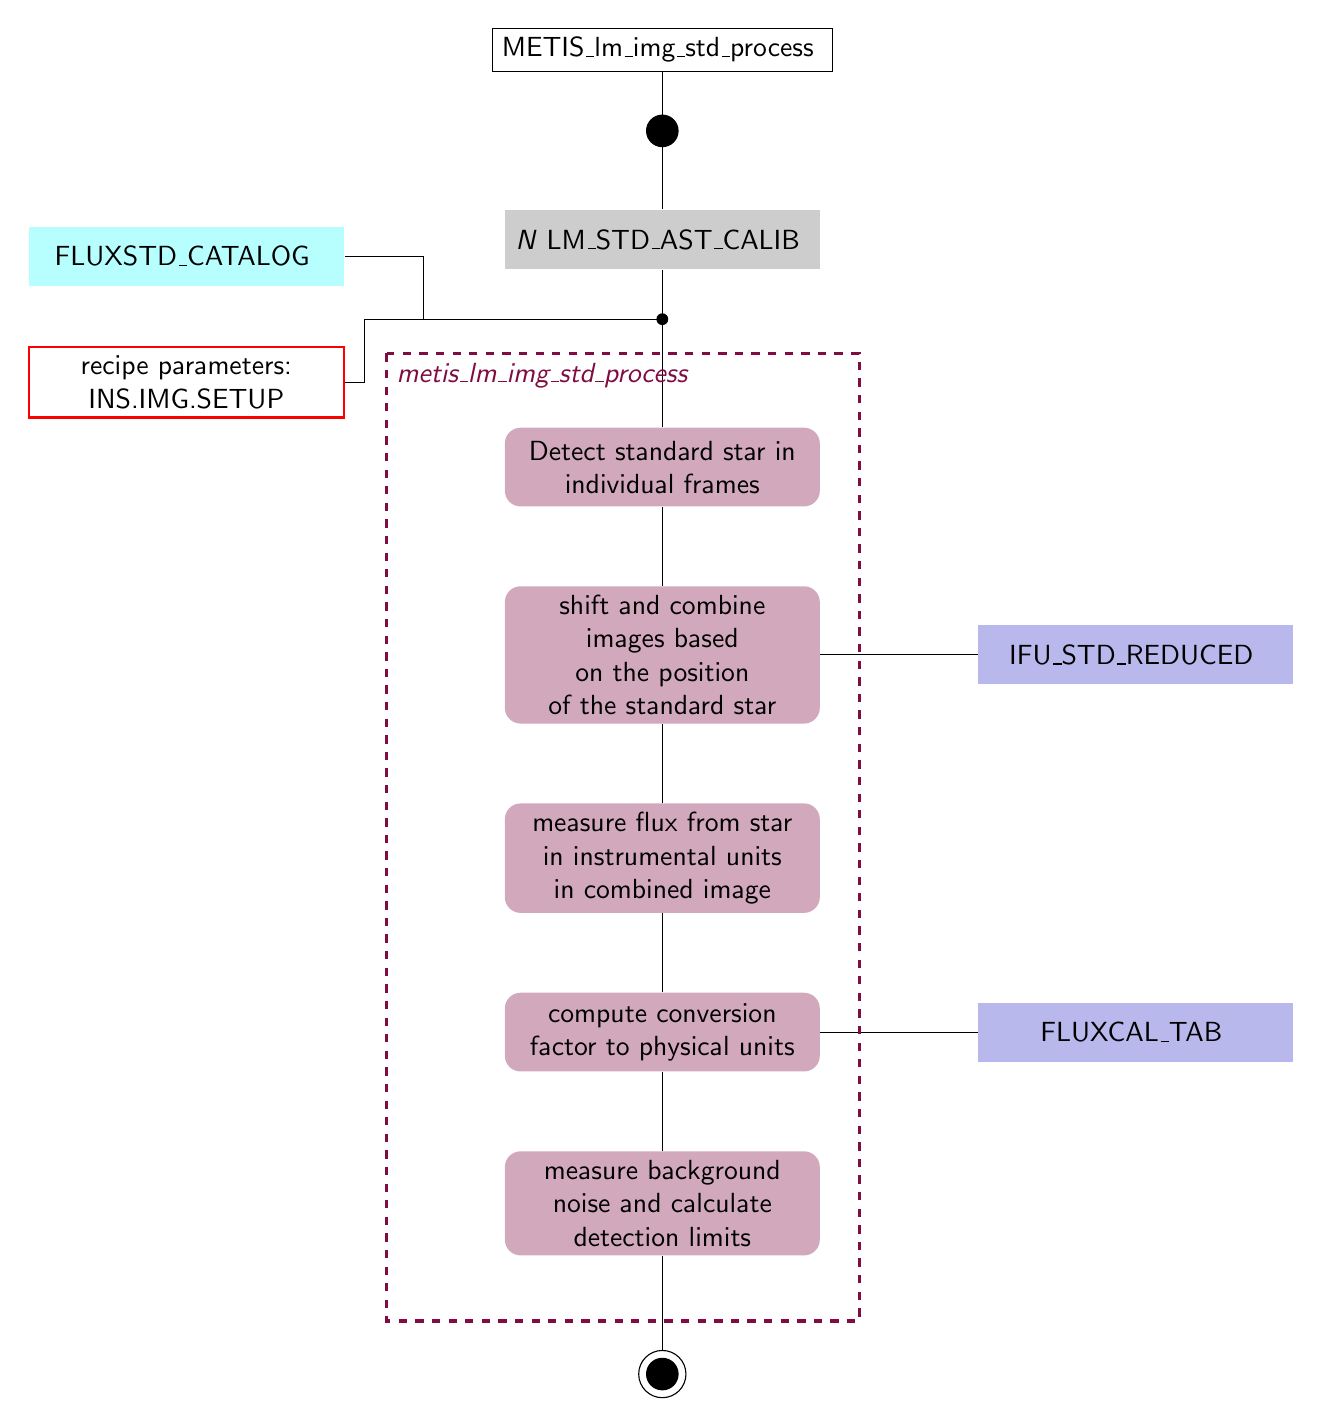
\begin{tikzpicture}
  [x=1cm,
  y=-1cm,
  align=center,
  node distance=2cm and 3cm]
  \sffamily

  %% Grid for orientation. Comment out for final figure!
% \draw[help lines, green](-8, 0) grid (8, 21);

  %%% Put workflow commands here:
  %% Main reduction workflow

  \node (template) [template]{%
   METIS\_lm\_img\_std\_process
  };

  \pic (start) [below=0.75cm of template] {start};

  \node (input) [below=0.75cm of start-m, input]{%
    \textsl{N} LM\_STD\_AST\_CALIB
  };

  \node (step1) [below=2cm of input, redstep]{%
    Detect standard star in\\
    individual frames
  };

  \node (step2)[below=1.cm of step1, redstep]{%
    shift and combine\\images
    based\\on the position\\of the
    standard star
  };

  \node (step3) [below=1.cm of step2, redstep]{%
    measure flux from star\\in instrumental units\\in combined image
  };

  \node (step4) [below=1.cm of step3, redstep]{%
    compute conversion\\factor to physical units
  };

  \node (step5) [below=1.cm of step4, redstep]{%
    measure background\\noise and calculate\\detection limits
  };

  %\node (step6) [below=1.cm of step5, %redstep]{%
  %  flux calibration
  %};

  \pic (stop) [below=1.5cm of step5]{stop};

  %% Connections
  \draw (template) -- (input);
  \draw (input) -- (step1);
  \draw (step1) -- (step2);
  \draw (step2) -- (step3);
  \draw (step3) -- (step4);
  \draw (step4) -- (step5);
  %\draw (step5) -- (step6);
  \draw (step5) -- (stop-t);

  %% Input
  \node (connectpers) [connection] at
  ($(input)!0.35!(step1)$) {};
  \node (persistence) [left=3.95cm of connectpers,yshift=0.8cm, external]{%
    FLUXSTD\_CATALOG
  };
  \draw (persistence.east) -- ++(1., 0) -- ++(0., 0.8) -- ++(3., 0);

  % Input for detector signature removal (step1)
  %\node (bpmin) [left=2cm of step1, yshift=0.8cm, calproduct]{%
  %  BADPIX\_MAP\_IFU
  %};
  %\draw (bpmin.east) -- ++(1., 0) -- ++(0., 0.6) -- ++(1., 0);

  %\node (darkin) [left=2cm of step1, calproduct] {%
  %  MASTER\_DARK\_IFU
  %};
  %\draw (darkin) -- (step1);

  %\node (flatin) [left=2cm of step1, yshift=-0.8cm, calproduct]{%
  %  MASTER\_FLAT\_IFU
  %};
  %\draw (flatin.east) -- ++(1., 0) -- ++(0., -0.6) -- ++(1., 0);

  % Input for rectification (step3)
  %\node (wavecal) [left=2cm of step3, yshift=0.4cm, calproduct]{%
  %  IFU\_WAVECAL
  %};
  %\draw (wavecal.east) -- ++(1., 0) -- %++(0., 0.3) -- ++(1., 0);

  %\node (distortion) [left=2cm of step3, yshift=-0.4cm, calproduct]{%
  %  IFU\_DISTORT\_TAB
  %};
  %\draw (distortion.east) -- ++(1., 0) -- ++(0., -0.3) -- ++(1., 0);

  % Further input
  \node (molecparams) [left=3.95cm of connectpers,yshift=-0.8cm, params]{%
    recipe parameters:\\INS.IMG.SETUP
  };
  \draw (molecparams.east) -- ++(0.25, 0) -- ++(0., -0.8) -- ++(3.75, 0);;

  %\node (stdcat) [left=2cm of step5, external] {%
   % FLUXSTD\_CATALOG
  %};
  %\draw (stdcat.east) -- (step5);

  %% Output
  %\node (connectreduced) [connection] at
 % ($(step5)!0.4!(stop-t)$) {};
  \node (reduced) [right=2cm of step2, calproduct]{%
    IFU\_STD\_REDUCED
  };
  \draw (step2) -- (reduced);

 % \node (connectfluxcal) [connection] at
 % ($(step5)!0.8!(stop-t)$) {};
  \node (fluxcal) [right=2cm of step4, calproduct]{%
    FLUXCAL\_TAB
  };
  \draw (step4) -- (fluxcal);

  %% Frame around recipe
  \draw [frame] ($(input)!0.5!(step1) - (3.5,0)$)
  rectangle ($(step5)!0.75!(stop-t) + (2.5,0)$);
  \node [framecolor, anchor=north west] at
  ($(input)!0.5!(step1) - (3.5, 0)$) {%
    \textsl{metis\_lm\_img\_std\_process}};

\end{tikzpicture}

% ADDING NEW DEFINITIONS -------------------------------------------- start
\definecolor{listingbg}{gray}{0.95}
\definecolor{darkgreen}{rgb}{0.0, 0.7, 0.0}
\definecolor{darkblue} {rgb}{0.0, 0.0, 0.7}
\definecolor{cyan} {rgb}{0.0, 0.4, 0.4}
\definecolor{darkred}  {rgb}{0.7, 0.0, 0.0}
\definecolor{darkorange}{rgb}{1.0, 0.49, 0.0}
\definecolor{violet}{rgb}{255, 0, 255}
\definecolor{turq}{rgb}{0.0, 0.7, 0.8}
\definecolor{fits}{rgb}{0.4, 0.1, 1}


\makeatletter
\lstdefinestyle{RAWstyle}{%
  basicstyle=\ttfamily\color{fits}%
  \lst@ifdisplaystyle\scriptsize\fi}

\lstdefinestyle{PARstyle}{%
  basicstyle=\ttfamily\color{cyan}%
  \lst@ifdisplaystyle\scriptsize\fi}

\lstdefinestyle{DRLstyle}{%
  basicstyle=\ttfamily\color{violet}%
  \lst@ifdisplaystyle\scriptsize\fi}

\lstdefinestyle{RECstyle}{%
  basicstyle=\ttfamily\color{darkgreen}%
  \lst@ifdisplaystyle\scriptsize\fi}

%% Write QC parameters like this: \QC{QC_SOMETHING_OR_OTHER}
\lstdefinestyle{QCstyle}{%
  basicstyle=\ttfamily\color{darkblue}%
  \lst@ifdisplaystyle\scriptsize\fi}

%% Write templates like this: \TPL{DARK_LM}
\lstdefinestyle{TPLstyle}{%
  basicstyle=\ttfamily\color{darkred}%
  \lst@ifdisplaystyle\scriptsize\fi}

%% Write products like this: \hyperref[dataitem:some_thing]{\PROD{SOME_THING}}
\lstdefinestyle{PRODstyle}{%
  basicstyle=\ttfamily\color{darkorange}%
  \lst@ifdisplaystyle\scriptsize\fi}

%% external calib files
\lstdefinestyle{EXTCALIBstyle}{%
  basicstyle=\ttfamily\color{Turquoise}%
  \lst@ifdisplaystyle\scriptsize\fi}

% static calib files
\lstdefinestyle{STATCALIBstyle}{%
  basicstyle=\ttfamily\color{teal}%
  \lst@ifdisplaystyle\scriptsize\fi}
\makeatother
